\PassOptionsToPackage{unicode=true}{hyperref} % options for packages loaded elsewhere
\PassOptionsToPackage{hyphens}{url}
%
\documentclass[
]{article}
\usepackage{lmodern}
\usepackage{amssymb,amsmath}
\usepackage{ifxetex,ifluatex}
\ifnum 0\ifxetex 1\fi\ifluatex 1\fi=0 % if pdftex
  \usepackage[T1]{fontenc}
  \usepackage[utf8]{inputenc}
  \usepackage{textcomp} % provides euro and other symbols
\else % if luatex or xelatex
  \usepackage{unicode-math}
  \defaultfontfeatures{Scale=MatchLowercase}
  \defaultfontfeatures[\rmfamily]{Ligatures=TeX,Scale=1}
\fi
% use upquote if available, for straight quotes in verbatim environments
\IfFileExists{upquote.sty}{\usepackage{upquote}}{}
\IfFileExists{microtype.sty}{% use microtype if available
  \usepackage[]{microtype}
  \UseMicrotypeSet[protrusion]{basicmath} % disable protrusion for tt fonts
}{}
\makeatletter
\@ifundefined{KOMAClassName}{% if non-KOMA class
  \IfFileExists{parskip.sty}{%
    \usepackage{parskip}
  }{% else
    \setlength{\parindent}{0pt}
    \setlength{\parskip}{6pt plus 2pt minus 1pt}}
}{% if KOMA class
  \KOMAoptions{parskip=half}}
\makeatother
\usepackage{xcolor}
\IfFileExists{xurl.sty}{\usepackage{xurl}}{} % add URL line breaks if available
\IfFileExists{bookmark.sty}{\usepackage{bookmark}}{\usepackage{hyperref}}
\hypersetup{
  pdfborder={0 0 0},
  breaklinks=true}
\urlstyle{same}  % don't use monospace font for urls
\usepackage[margin=1in]{geometry}
\usepackage{color}
\usepackage{fancyvrb}
\newcommand{\VerbBar}{|}
\newcommand{\VERB}{\Verb[commandchars=\\\{\}]}
\DefineVerbatimEnvironment{Highlighting}{Verbatim}{commandchars=\\\{\}}
% Add ',fontsize=\small' for more characters per line
\usepackage{framed}
\definecolor{shadecolor}{RGB}{248,248,248}
\newenvironment{Shaded}{\begin{snugshade}}{\end{snugshade}}
\newcommand{\AlertTok}[1]{\textcolor[rgb]{0.94,0.16,0.16}{#1}}
\newcommand{\AnnotationTok}[1]{\textcolor[rgb]{0.56,0.35,0.01}{\textbf{\textit{#1}}}}
\newcommand{\AttributeTok}[1]{\textcolor[rgb]{0.77,0.63,0.00}{#1}}
\newcommand{\BaseNTok}[1]{\textcolor[rgb]{0.00,0.00,0.81}{#1}}
\newcommand{\BuiltInTok}[1]{#1}
\newcommand{\CharTok}[1]{\textcolor[rgb]{0.31,0.60,0.02}{#1}}
\newcommand{\CommentTok}[1]{\textcolor[rgb]{0.56,0.35,0.01}{\textit{#1}}}
\newcommand{\CommentVarTok}[1]{\textcolor[rgb]{0.56,0.35,0.01}{\textbf{\textit{#1}}}}
\newcommand{\ConstantTok}[1]{\textcolor[rgb]{0.00,0.00,0.00}{#1}}
\newcommand{\ControlFlowTok}[1]{\textcolor[rgb]{0.13,0.29,0.53}{\textbf{#1}}}
\newcommand{\DataTypeTok}[1]{\textcolor[rgb]{0.13,0.29,0.53}{#1}}
\newcommand{\DecValTok}[1]{\textcolor[rgb]{0.00,0.00,0.81}{#1}}
\newcommand{\DocumentationTok}[1]{\textcolor[rgb]{0.56,0.35,0.01}{\textbf{\textit{#1}}}}
\newcommand{\ErrorTok}[1]{\textcolor[rgb]{0.64,0.00,0.00}{\textbf{#1}}}
\newcommand{\ExtensionTok}[1]{#1}
\newcommand{\FloatTok}[1]{\textcolor[rgb]{0.00,0.00,0.81}{#1}}
\newcommand{\FunctionTok}[1]{\textcolor[rgb]{0.00,0.00,0.00}{#1}}
\newcommand{\ImportTok}[1]{#1}
\newcommand{\InformationTok}[1]{\textcolor[rgb]{0.56,0.35,0.01}{\textbf{\textit{#1}}}}
\newcommand{\KeywordTok}[1]{\textcolor[rgb]{0.13,0.29,0.53}{\textbf{#1}}}
\newcommand{\NormalTok}[1]{#1}
\newcommand{\OperatorTok}[1]{\textcolor[rgb]{0.81,0.36,0.00}{\textbf{#1}}}
\newcommand{\OtherTok}[1]{\textcolor[rgb]{0.56,0.35,0.01}{#1}}
\newcommand{\PreprocessorTok}[1]{\textcolor[rgb]{0.56,0.35,0.01}{\textit{#1}}}
\newcommand{\RegionMarkerTok}[1]{#1}
\newcommand{\SpecialCharTok}[1]{\textcolor[rgb]{0.00,0.00,0.00}{#1}}
\newcommand{\SpecialStringTok}[1]{\textcolor[rgb]{0.31,0.60,0.02}{#1}}
\newcommand{\StringTok}[1]{\textcolor[rgb]{0.31,0.60,0.02}{#1}}
\newcommand{\VariableTok}[1]{\textcolor[rgb]{0.00,0.00,0.00}{#1}}
\newcommand{\VerbatimStringTok}[1]{\textcolor[rgb]{0.31,0.60,0.02}{#1}}
\newcommand{\WarningTok}[1]{\textcolor[rgb]{0.56,0.35,0.01}{\textbf{\textit{#1}}}}
\usepackage{graphicx,grffile}
\makeatletter
\def\maxwidth{\ifdim\Gin@nat@width>\linewidth\linewidth\else\Gin@nat@width\fi}
\def\maxheight{\ifdim\Gin@nat@height>\textheight\textheight\else\Gin@nat@height\fi}
\makeatother
% Scale images if necessary, so that they will not overflow the page
% margins by default, and it is still possible to overwrite the defaults
% using explicit options in \includegraphics[width, height, ...]{}
\setkeys{Gin}{width=\maxwidth,height=\maxheight,keepaspectratio}
\setlength{\emergencystretch}{3em}  % prevent overfull lines
\providecommand{\tightlist}{%
  \setlength{\itemsep}{0pt}\setlength{\parskip}{0pt}}
\setcounter{secnumdepth}{-2}
% Redefines (sub)paragraphs to behave more like sections
\ifx\paragraph\undefined\else
  \let\oldparagraph\paragraph
  \renewcommand{\paragraph}[1]{\oldparagraph{#1}\mbox{}}
\fi
\ifx\subparagraph\undefined\else
  \let\oldsubparagraph\subparagraph
  \renewcommand{\subparagraph}[1]{\oldsubparagraph{#1}\mbox{}}
\fi

% set default figure placement to htbp
\makeatletter
\def\fps@figure{htbp}
\makeatother

\usepackage{pdflscape}
\usepackage{booktabs}
\usepackage{xcolor}
\usepackage{colortbl}
\usepackage{graphicx}
\usepackage{booktabs}
\usepackage{longtable}
\usepackage{array}
\usepackage{multirow}
\usepackage{wrapfig}
\usepackage{float}
\usepackage{colortbl}
\usepackage{pdflscape}
\usepackage{tabu}
\usepackage{threeparttable}
\usepackage{threeparttablex}
\usepackage[normalem]{ulem}
\usepackage{makecell}
\usepackage{xcolor}

\author{}
\date{\vspace{-2.5em}}

\begin{document}

\begin{verbatim}
## -- Attaching packages --------------------------------------- tidyverse 1.3.0 --
\end{verbatim}

\begin{verbatim}
## v ggplot2 3.3.2     v purrr   0.3.4
## v tibble  3.0.4     v dplyr   1.0.0
## v tidyr   1.1.2     v stringr 1.4.0
## v readr   1.4.0     v forcats 0.5.0
\end{verbatim}

\begin{verbatim}
## -- Conflicts ------------------------------------------ tidyverse_conflicts() --
## x dplyr::filter() masks stats::filter()
## x dplyr::lag()    masks stats::lag()
\end{verbatim}

\begin{verbatim}
## 
## Attaching package: 'scales'
\end{verbatim}

\begin{verbatim}
## The following object is masked from 'package:purrr':
## 
##     discard
\end{verbatim}

\begin{verbatim}
## The following object is masked from 'package:readr':
## 
##     col_factor
\end{verbatim}

\begin{verbatim}
## 
## Attaching package: 'zoo'
\end{verbatim}

\begin{verbatim}
## The following objects are masked from 'package:base':
## 
##     as.Date, as.Date.numeric
\end{verbatim}

\begin{verbatim}
## 
## Attaching package: 'kableExtra'
\end{verbatim}

\begin{verbatim}
## The following object is masked from 'package:dplyr':
## 
##     group_rows
\end{verbatim}

\begin{verbatim}
## 
## Attaching package: 'lubridate'
\end{verbatim}

\begin{verbatim}
## The following objects are masked from 'package:base':
## 
##     date, intersect, setdiff, union
\end{verbatim}

\begin{verbatim}
## `summarise()` regrouping output by 'Quarantine', 'Location2' (override with `.groups` argument)
\end{verbatim}

\begin{verbatim}
## `summarise()` regrouping output by 'Location2' (override with `.groups` argument)
## `summarise()` regrouping output by 'Location2' (override with `.groups` argument)
## `summarise()` regrouping output by 'Location2' (override with `.groups` argument)
\end{verbatim}

\begin{verbatim}
## `summarise()` ungrouping output (override with `.groups` argument)
\end{verbatim}

\begin{verbatim}
## `summarise()` regrouping output by 'Isolated' (override with `.groups` argument)
\end{verbatim}

\begin{verbatim}
## `summarise()` ungrouping output (override with `.groups` argument)
## `summarise()` ungrouping output (override with `.groups` argument)
## `summarise()` ungrouping output (override with `.groups` argument)
## `summarise()` ungrouping output (override with `.groups` argument)
\end{verbatim}

\begin{verbatim}
## `summarise()` regrouping output by 'Test_Date' (override with `.groups` argument)
\end{verbatim}

\begin{verbatim}
## `summarise()` ungrouping output (override with `.groups` argument)
## `summarise()` ungrouping output (override with `.groups` argument)
## `summarise()` ungrouping output (override with `.groups` argument)
## `summarise()` ungrouping output (override with `.groups` argument)
## `summarise()` ungrouping output (override with `.groups` argument)
## `summarise()` ungrouping output (override with `.groups` argument)
## `summarise()` ungrouping output (override with `.groups` argument)
## `summarise()` ungrouping output (override with `.groups` argument)
## `summarise()` ungrouping output (override with `.groups` argument)
\end{verbatim}


\includegraphics{Logo-GC-Red-Background-Stretched.jpg}\\

\hypertarget{grace-college-internal-covid-19-data}{%
\section{Grace College Internal COVID-19
Data}\label{grace-college-internal-covid-19-data}}

\hypertarget{compiled-by-dr.-ryan-johnson-using-contact-tracing-data-from-laura-green-and-nicole-gibson-as-well-as-testing-data-from-the-state-of-indiana.}{%
\subsection{Compiled by Dr.~Ryan Johnson using contact tracing data from
Laura Green and Nicole Gibson, as well as testing data from the state of
Indiana.}\label{compiled-by-dr.-ryan-johnson-using-contact-tracing-data-from-laura-green-and-nicole-gibson-as-well-as-testing-data-from-the-state-of-indiana.}}

\hypertarget{last-updated-wednesday-january-13-2021-at-1037am}{%
\subsubsection{Last updated Wednesday, January 13, 2021, at
10:37AM}\label{last-updated-wednesday-january-13-2021-at-1037am}}

\vspace{2 in}

Notes and Irregularities:

\begin{itemize}
\tightlist
\item
  Quarantined from international travel are a subcategory of students
  quarantined at Grace.
\end{itemize}

\newpage

\hypertarget{cases}{%
\section{Cases}\label{cases}}

\hypertarget{confirmed-cases-among-students}{%
\subsubsection{Confirmed Cases Among
Students}\label{confirmed-cases-among-students}}

As of yesterday, Grace College had

\begin{Shaded}
\begin{Highlighting}[]
\NormalTok{CS_Tab }\OperatorTok
\StringTok{  }\KeywordTok{select}\NormalTok{(Type, Total, at_Home, at_Grace)}\OperatorTok
\StringTok{  }\NormalTok{kableExtra}\OperatorTok{::}\KeywordTok{kable}\NormalTok{(}\DataTypeTok{caption =} \StringTok{"Student Cases"}\NormalTok{, }\DataTypeTok{booktabs =} \OtherTok{TRUE}\NormalTok{, }\DataTypeTok{format =} \StringTok{"latex"}\NormalTok{) }\OperatorTok
\StringTok{  }\KeywordTok{kable_styling}\NormalTok{(}\DataTypeTok{latex_options =} \StringTok{"striped"}\NormalTok{)}\OperatorTok
\StringTok{  }\KeywordTok{kable_styling}\NormalTok{(}\DataTypeTok{latex_options =} \StringTok{"hold_position"}\NormalTok{)}
\end{Highlighting}
\end{Shaded}

\begin{table}[!h]

\caption{\label{tab:unnamed-chunk-2}Student Cases}
\centering
\begin{tabular}[t]{lrrr}
\toprule
Type & Total & at\_Home & at\_Grace\\
\midrule
\cellcolor{gray!6}{Active on Tue Jan 12} & \cellcolor{gray!6}{0} & \cellcolor{gray!6}{0} & \cellcolor{gray!6}{0}\\
Spring Semester Total & 0 & 0 & 0\\
\cellcolor{gray!6}{20-21 Academic Year Total} & \cellcolor{gray!6}{111} & \cellcolor{gray!6}{72} & \cellcolor{gray!6}{39}\\
\bottomrule
\end{tabular}
\end{table}

\hypertarget{confirmed-cases-among-employees}{%
\subsubsection{Confirmed Cases Among
Employees}\label{confirmed-cases-among-employees}}

As of yesterday, Grace College had

\begin{table}[!h]

\caption{\label{tab:unnamed-chunk-4}Employee Cases}
\centering
\begin{tabular}[t]{lr}
\toprule
Type & Cases\\
\midrule
\cellcolor{gray!6}{Active on Tue Jan 12} & \cellcolor{gray!6}{2}\\
Spring Semester Total & 2\\
\cellcolor{gray!6}{20-21 Academic Year Total} & \cellcolor{gray!6}{37}\\
\bottomrule
\end{tabular}
\end{table}

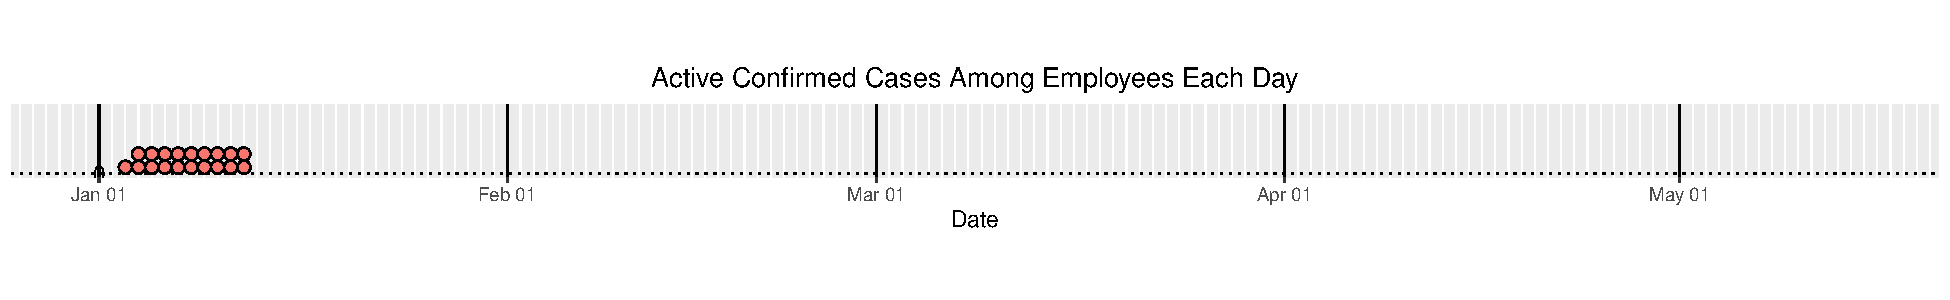
\includegraphics{Grace_internal4_files/figure-latex/unnamed-chunk-5-1.pdf}

\newpage

\hypertarget{isolated}{%
\section{Isolated}\label{isolated}}

\hypertarget{isolated-students}{%
\subsubsection{Isolated Students}\label{isolated-students}}

\begin{table}[!h]

\caption{\label{tab:unnamed-chunk-6}Student Isolations}
\centering
\begin{tabular}[t]{lrrr}
\toprule
Type & Total & at\_Home & at\_Grace\\
\midrule
\cellcolor{gray!6}{Active on Tue Jan 12} & \cellcolor{gray!6}{0} & \cellcolor{gray!6}{0} & \cellcolor{gray!6}{0}\\
Spring Semester Total & 0 & 0 & 0\\
\cellcolor{gray!6}{20-21 Academic Year Total} & \cellcolor{gray!6}{204} & \cellcolor{gray!6}{140} & \cellcolor{gray!6}{64}\\
20-21 Academic Year Unique Students & 197 & 133 & 64\\
\bottomrule
\end{tabular}
\end{table}

\hypertarget{isolated-employees}{%
\subsubsection{Isolated Employees}\label{isolated-employees}}

As of yesterday, Grace College had

\begin{table}[!h]

\caption{\label{tab:unnamed-chunk-8}Employee Isolations}
\centering
\begin{tabular}[t]{lr}
\toprule
Type & Isolated\\
\midrule
\cellcolor{gray!6}{Active on Tue Jan 12} & \cellcolor{gray!6}{3}\\
Spring Semester Total & 3\\
\cellcolor{gray!6}{20-21 Academic Year Total} & \cellcolor{gray!6}{55}\\
\bottomrule
\end{tabular}
\end{table}

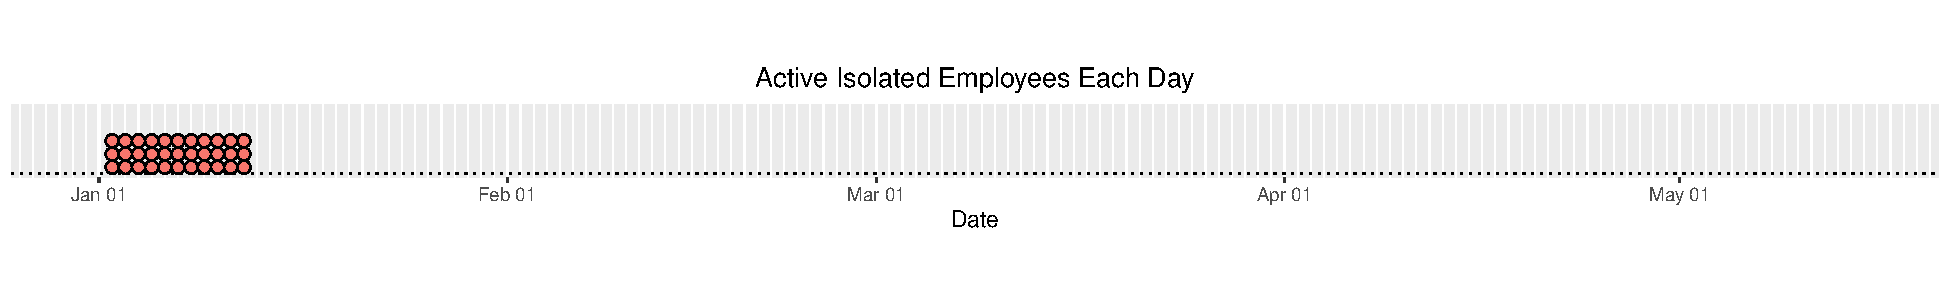
\includegraphics{Grace_internal4_files/figure-latex/unnamed-chunk-9-1.pdf}

\newpage

\hypertarget{quarantined}{%
\section{Quarantined}\label{quarantined}}

\hypertarget{quarantined-students}{%
\subsubsection{Quarantined Students}\label{quarantined-students}}

In the table below, \texttt{from\_travel} is a subcategory of
\texttt{at\_Grace}.

\begin{table}[!h]

\caption{\label{tab:unnamed-chunk-10}Student Quarantines}
\centering
\begin{tabular}[t]{lrrrr}
\toprule
Type & Total & at\_Home & at\_Grace & from\_travel\\
\midrule
\cellcolor{gray!6}{Active on Tue Jan 12} & \cellcolor{gray!6}{15} & \cellcolor{gray!6}{0} & \cellcolor{gray!6}{15} & \cellcolor{gray!6}{15}\\
Spring Semester Total & 15 & 0 & 15 & 15\\
\cellcolor{gray!6}{20-21 Academic Year Total} & \cellcolor{gray!6}{486} & \cellcolor{gray!6}{345} & \cellcolor{gray!6}{140} & \cellcolor{gray!6}{40}\\
20-21 Academic Year Unique Students & 448 & 316 & 131 & 34\\
\bottomrule
\end{tabular}
\end{table}

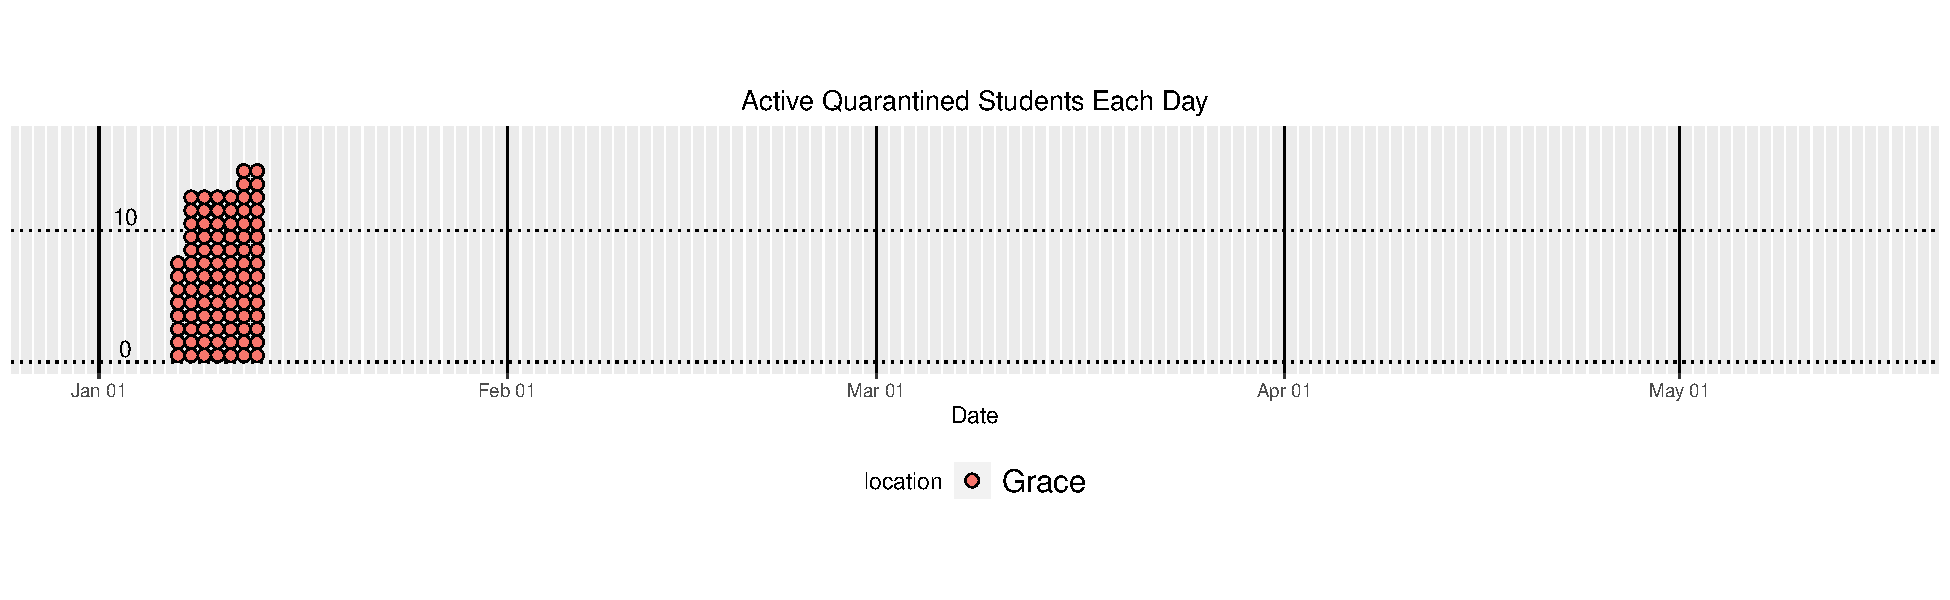
\includegraphics{Grace_internal4_files/figure-latex/unnamed-chunk-11-1.pdf}

\hypertarget{quarantined-employees}{%
\subsubsection{Quarantined Employees}\label{quarantined-employees}}

As of yesterday, Grace College had

\begin{table}[!h]

\caption{\label{tab:unnamed-chunk-12}Employee Quarantines}
\centering
\begin{tabular}[t]{lr}
\toprule
Type & Quarantine\\
\midrule
\cellcolor{gray!6}{Active on Tue Jan 12} & \cellcolor{gray!6}{1}\\
Spring Semester Total & 2\\
\cellcolor{gray!6}{20-21 Academic Year Total} & \cellcolor{gray!6}{58}\\
\bottomrule
\end{tabular}
\end{table}

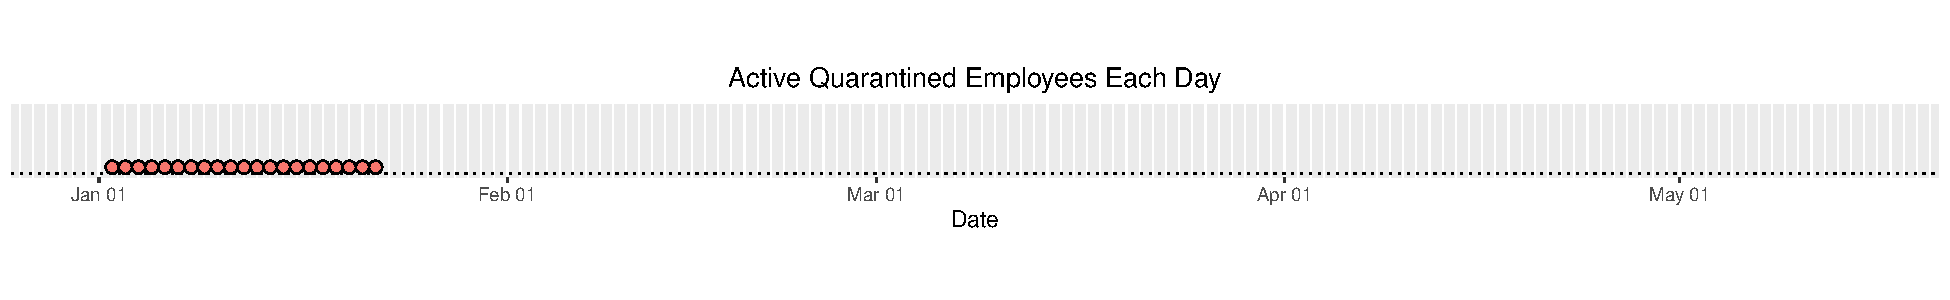
\includegraphics{Grace_internal4_files/figure-latex/unnamed-chunk-13-1.pdf}

\newpage

\newpage

\hypertarget{kosciusko-county}{%
\section{Kosciusko County}\label{kosciusko-county}}

Kosciusko County has had

\begin{itemize}
\tightlist
\item
  87 cases per day the past week.
\item
  6337 total confirmed cases.
\end{itemize}

\hypertarget{cases---kosciusko}{%
\subsubsection{Cases - Kosciusko}\label{cases---kosciusko}}

\begin{verbatim}
## `geom_smooth()` using method = 'loess' and formula 'y ~ x'
\end{verbatim}

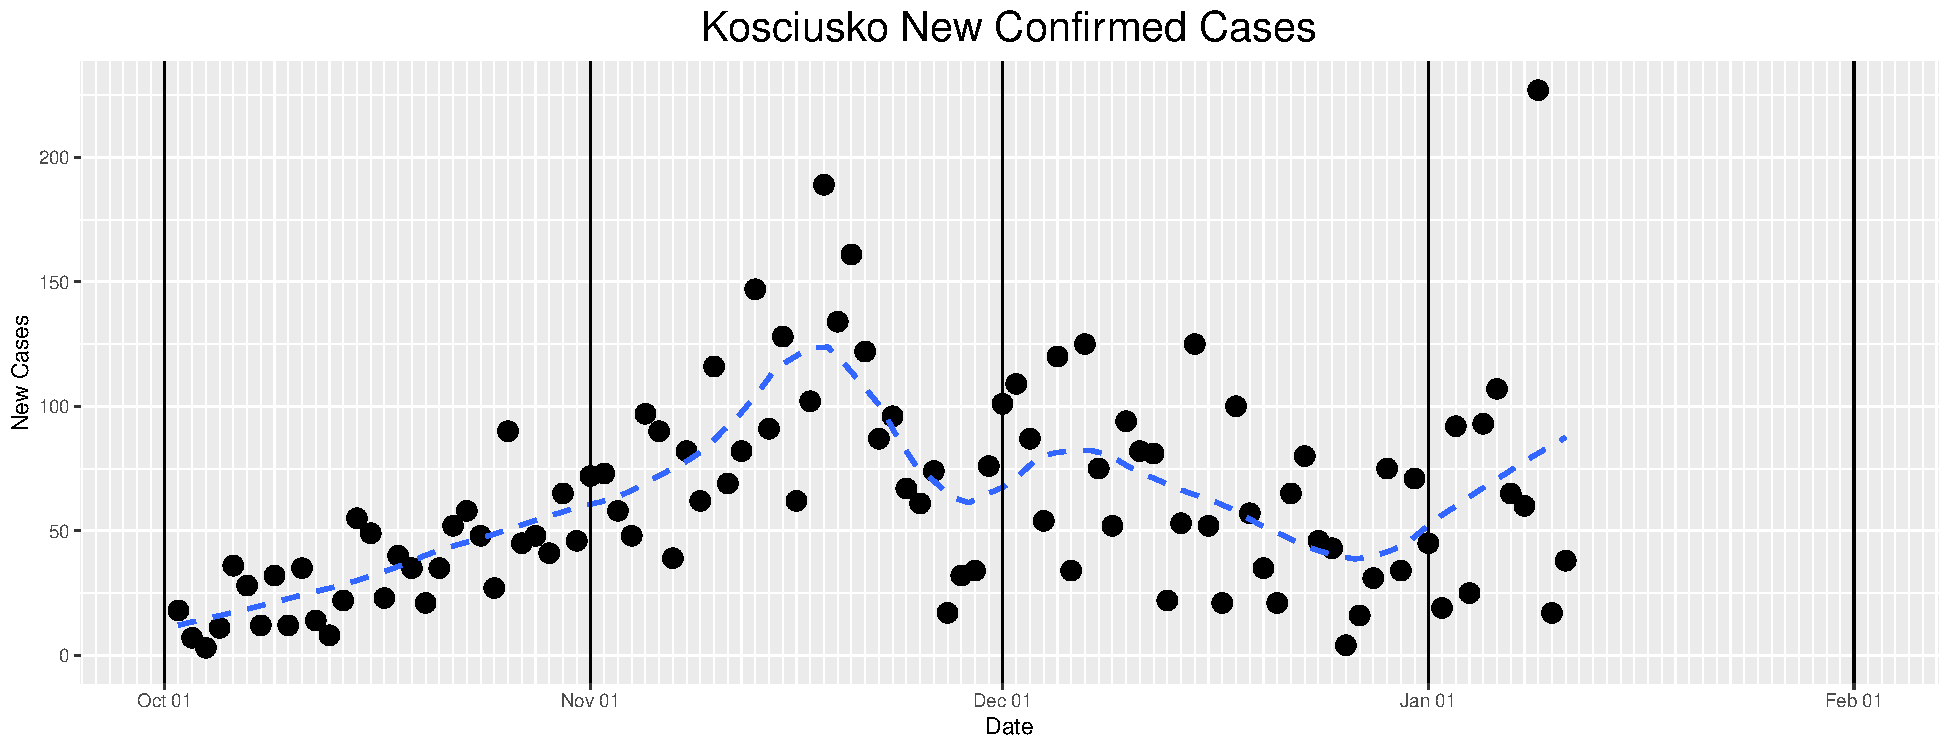
\includegraphics{Grace_internal4_files/figure-latex/unnamed-chunk-15-1.pdf}

\hypertarget{positivity---kosciusko}{%
\subsubsection{Positivity - Kosciusko}\label{positivity---kosciusko}}

Kosciusko County has had 32.1\% 7-day positivity rate for unique
indiviudals as of January 05.

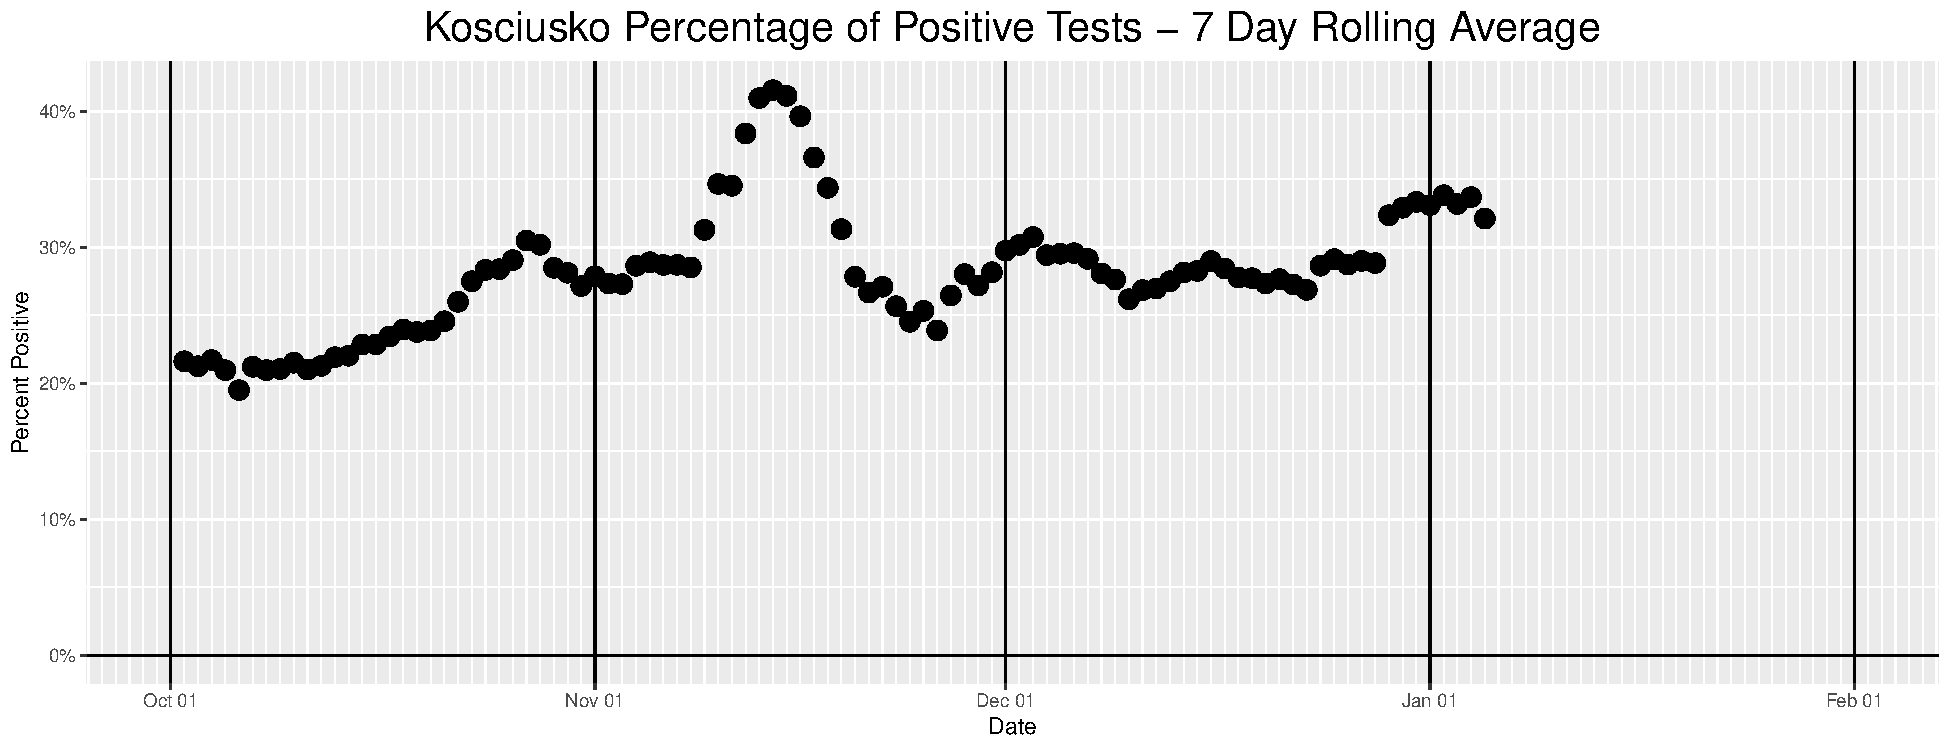
\includegraphics{Grace_internal4_files/figure-latex/unnamed-chunk-16-1.pdf}

\newpage

\hypertarget{indiana}{%
\section{Indiana}\label{indiana}}

The total case numbers below are multiplied by
\(\frac{\text{Kos pop}}{\text{Ind pop}} = \frac{79456}{6732000} = 0.01180273\),
so that it is easier to compare Kosciusko numbers to the average Indiana
county.

Indiana has had

\begin{itemize}
\tightlist
\item
  5360.4 cases per day the past week (normalized 63.3).
\item
  447,991 total confirmed cases (normalized 5287.5).
\end{itemize}

\hypertarget{cases---indiana}{%
\subsubsection{Cases - Indiana}\label{cases---indiana}}

\begin{verbatim}
## `geom_smooth()` using method = 'loess' and formula 'y ~ x'
\end{verbatim}

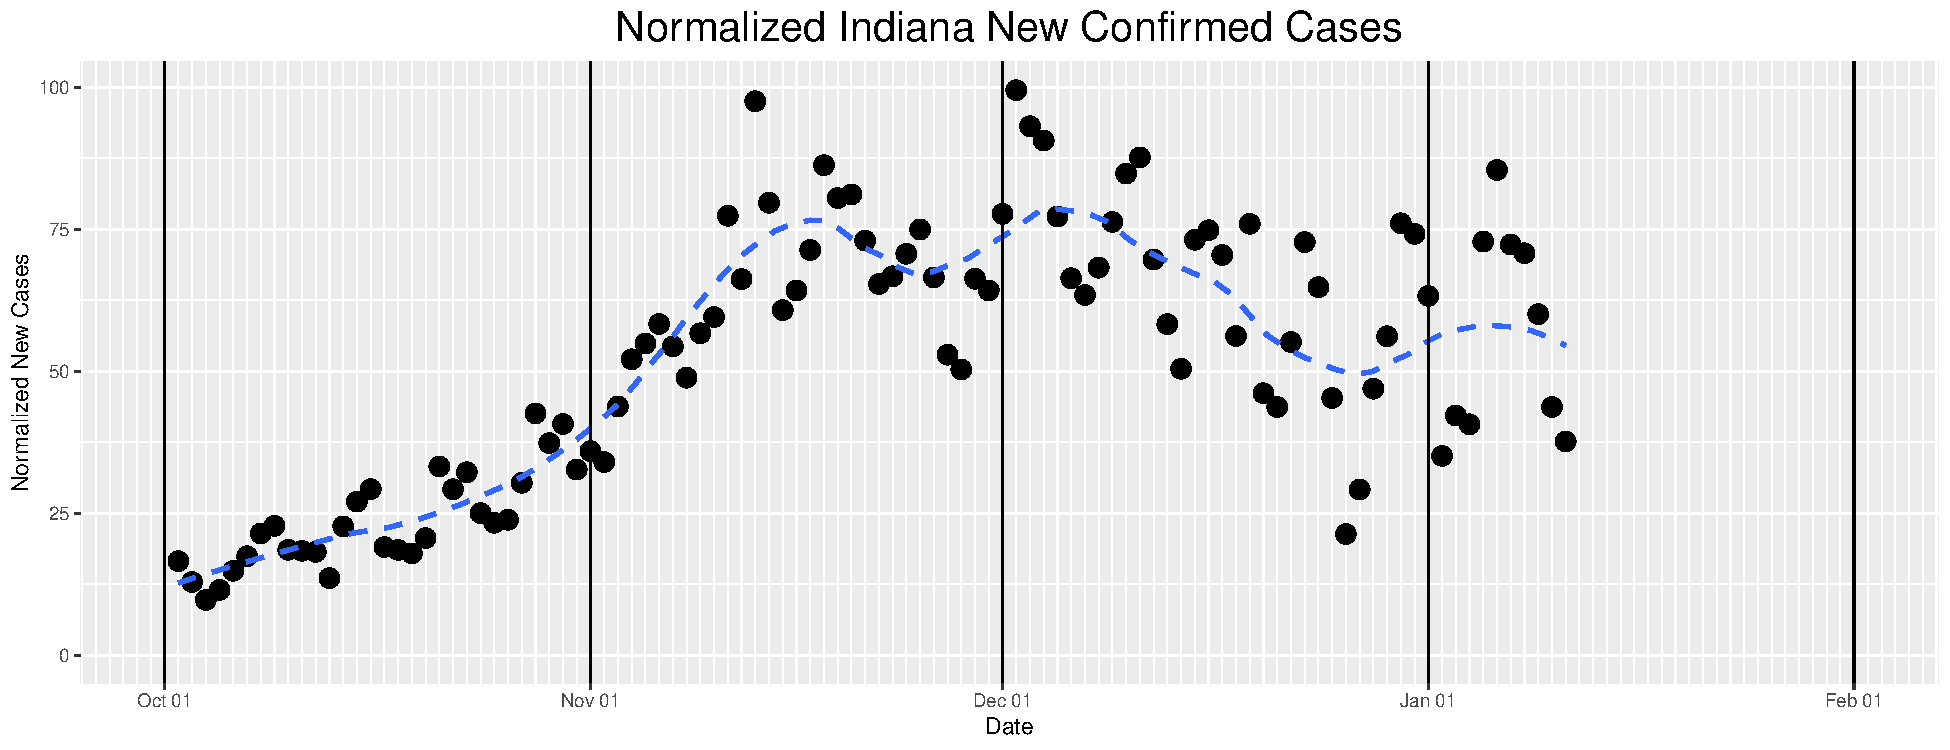
\includegraphics{Grace_internal4_files/figure-latex/unnamed-chunk-17-1.pdf}

\hypertarget{positivity---indiana}{%
\subsubsection{Positivity - Indiana}\label{positivity---indiana}}

Indiana reports a 15\% 7-day positivity rate for all tests as of January
05.

\begin{verbatim}
## `geom_smooth()` using method = 'loess' and formula 'y ~ x'
\end{verbatim}

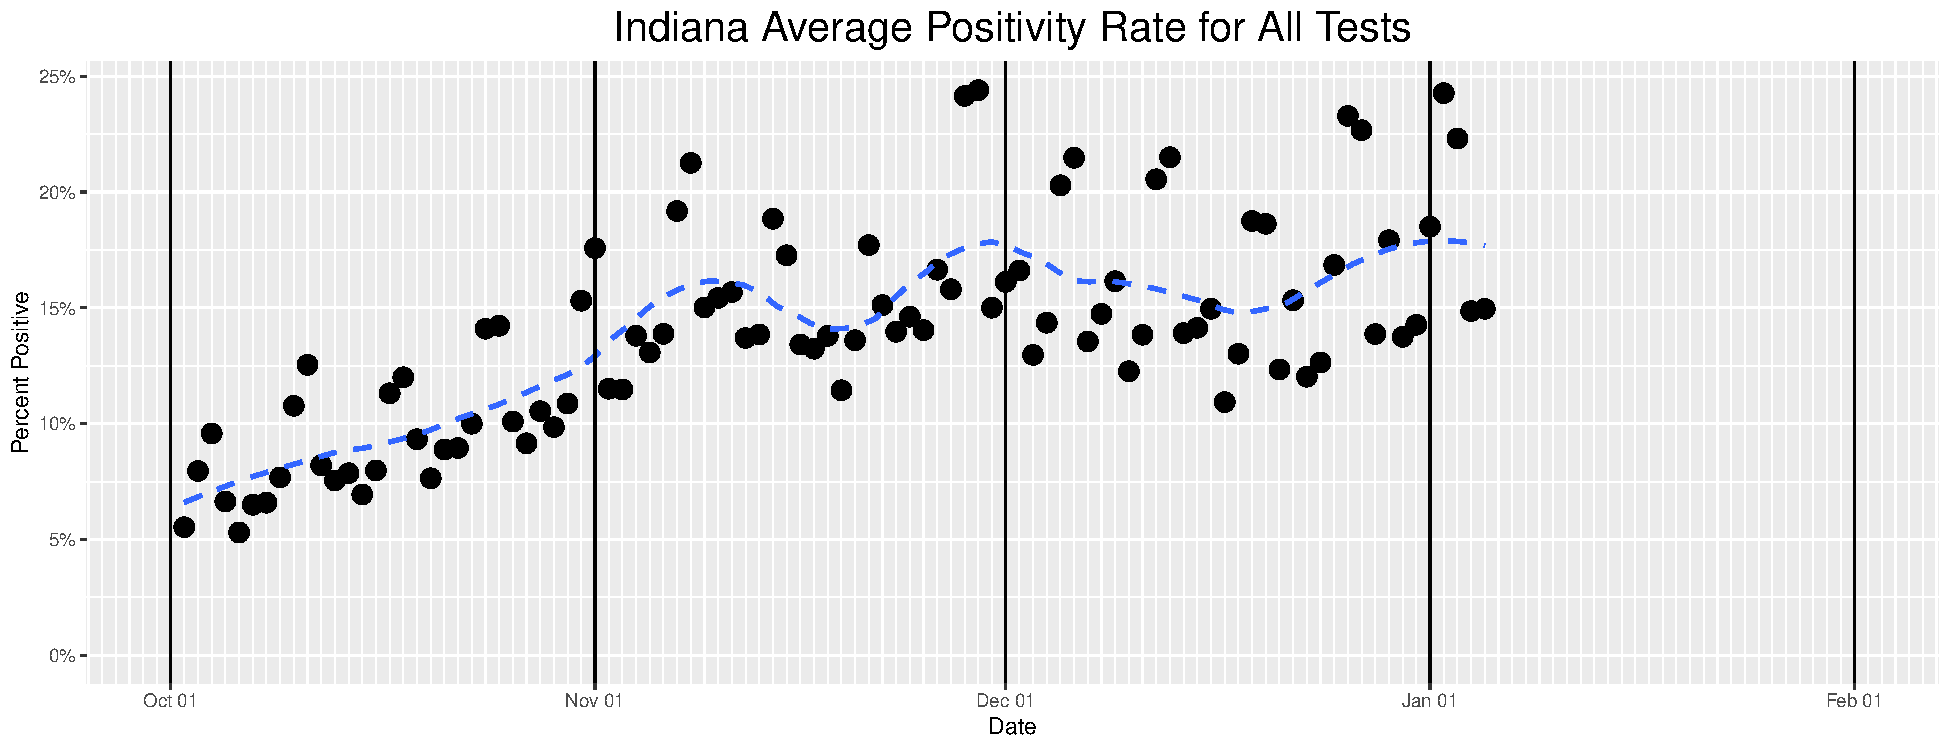
\includegraphics{Grace_internal4_files/figure-latex/unnamed-chunk-18-1.pdf}

\newpage

\hypertarget{indiana-map}{%
\section{Indiana Map}\label{indiana-map}}

The map below displays the cases per 100,000 per day averaged over the
past week and the positivity rate for unique individuals averaged over
the previous week. The coloring scheme is relative, it colors the best
county white and the worst county red.

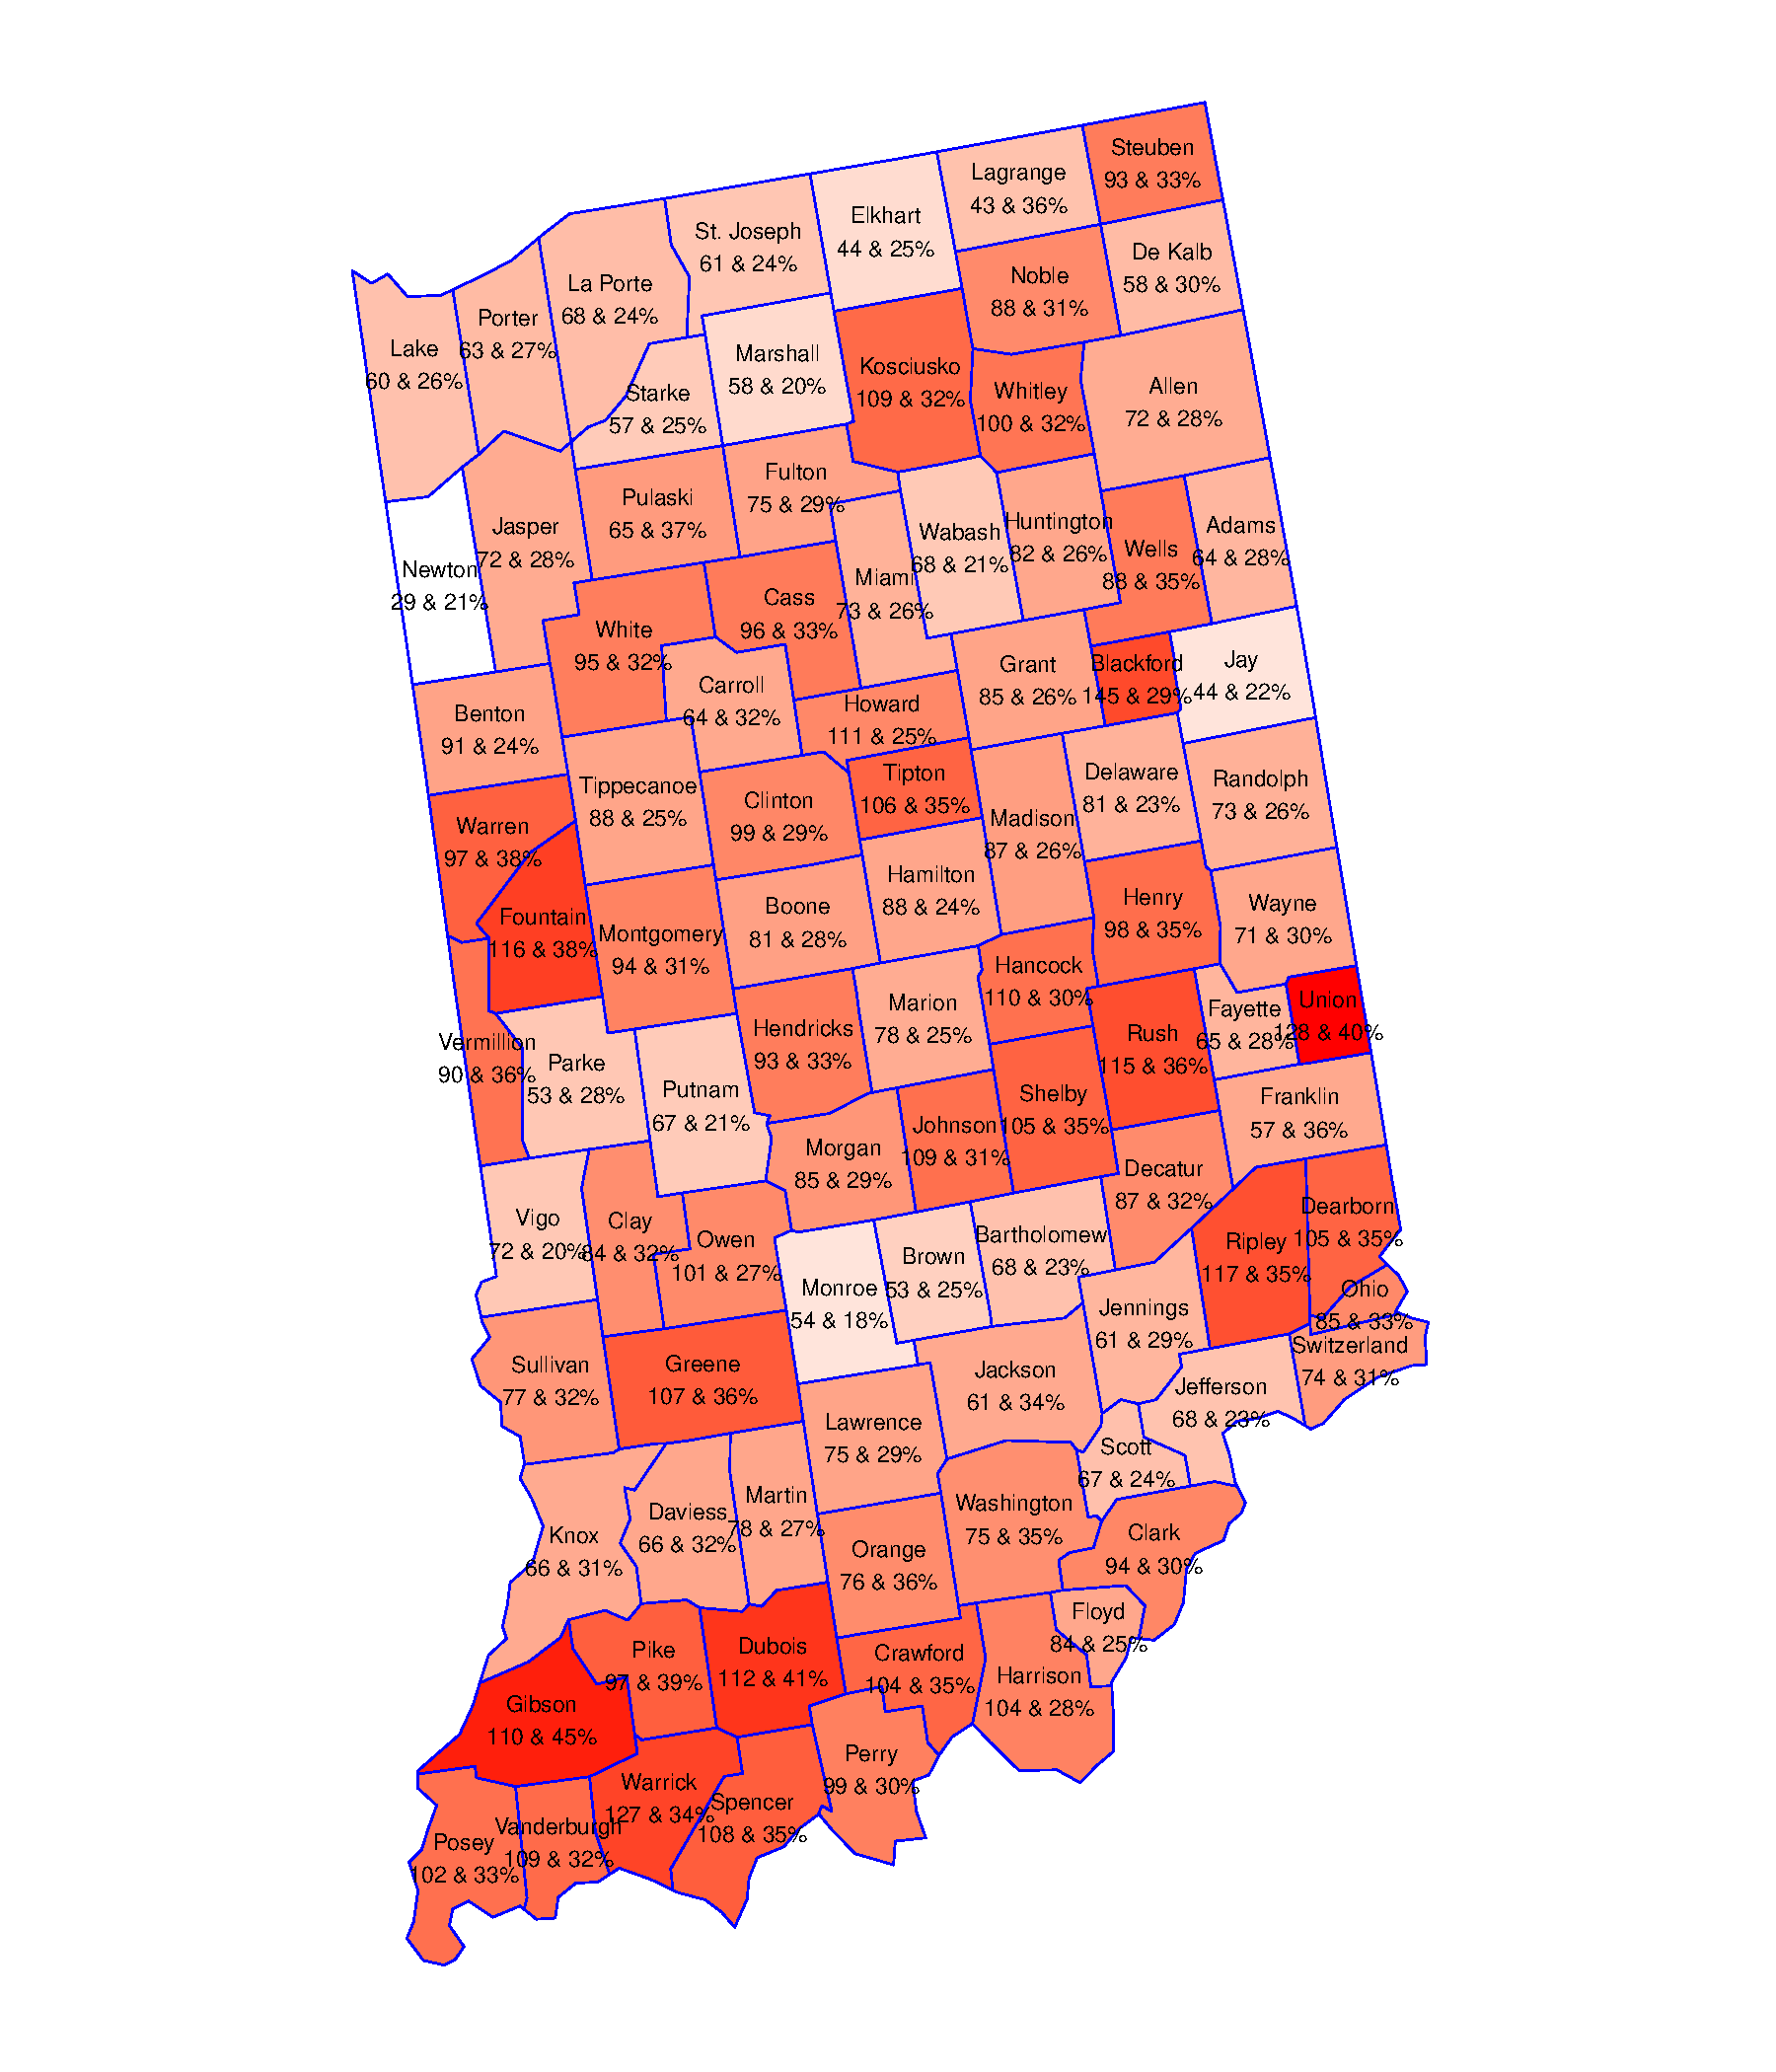
\includegraphics{Grace_internal4_files/figure-latex/unnamed-chunk-19-1.pdf}

\end{document}
